\documentclass[refman]{article}

\usepackage[utf8]{inputenc}
\usepackage[english]{babel}

\usepackage{colortbl}
\usepackage{epigraph}
\usepackage{fancyhdr}
\usepackage{graphicx}
\usepackage{hhline}
%\usepackage{biblatex}
\usepackage{wrapfig}

\usepackage[procnames]{listings}
\usepackage{longtable}
\usepackage{tikz}
\usepackage{subcaption}
\usepackage{xcolor}
\usepackage{wrapfig}
\usepackage[nottoc,numbib]{tocbibind}
%
%\usepackage[T1]{fontenc}
\usepackage{lmodern}

\usepackage{amsfonts}
\usepackage{amsmath}
\usepackage{amsthm}
\usepackage{mathtools}

\usepackage{geometry}
 \geometry{
 a4paper,
 left=30mm,
 top=30mm,
 }
\pagestyle{fancy}

\newcommand{\idx}{\text{idx}}

\DeclarePairedDelimiter\ceil{\lceil}{\rceil}
\DeclarePairedDelimiter\floor{\lfloor}{\rfloor}

\theoremstyle{definition}
\newtheorem*{formula}{Formula}

\usepackage[document]{ragged2e}

\begin{document}
\section{Introduction: Setting the Stage}

This protocol discusses a numerical approach to solve second order partial differential equations\footnote{This is sometimes referred as Laplace's equation.}. To draw inspiration from a physical example for this mathematical problem, visualize a two dimensional space in which a string is fixed at both ends and a force, such as gravity, acting on the said string. From the Newtonian mechanics, we have the equation
\begin{align*}
	F = ma \text{.}
\end{align*}
In the above equation, \(F\) denotes the force, and \(a\) is the acceleration which is just the second derivative of the location or in our case the displacement which can be thought as a function of the points of the string, \(u(x)\). If we na{\"i}vely set the mass \(m = 1\), we have\footnote{The minus sign in front of \(u\) arises from convention. We have also replaced \(F\) with \(f\) to adhere to a more mathematical standard.}
\begin{align*}
	f(x) = - u''(x) \text{.}
\end{align*}
Assuming the values for the function \(f\) is known we want to describe a procedure how to numerically compute the solution for \(u\). Ultimately, we will do this by approximating the second partial derivative with Taylor polynomials and constructing a linear transformation which maps a vector containing \(u\) for every evaluated point \(x_i\) to a vector which encodes the values of \(f\).
However, this protocol is meant to be a preparatory piece and while we will describe in detail the construction of the matrix for the linear transformation, we will not discuss how to solve the system for \(u\).
\section{Theory}

Before we continue with our endeavour, it is a good idea to reiterate fundamental results of linear algebra.

\subsection{LU Decomposition}
\section{Experiments}
\subsection{Optimal Omega}

We first want to focus on finding an optimal value for \(\omega\) to minimize the error given a practical termination condition (see user manual). If we take \(d = 1\) and \(n = 10\), then \(\omega_{\text{opt}}\) is between \(1.2\) and \(1.3\). Interestingly, if we fix \(n\), but change the dimension, the optimal value for \(\omega\) is still between \(1.2\) and \(1.3\), therefore, we can conjecture that \(\omega_\text{opt}\) is not dependent on \(d\). However, it is most definitely dependent on \(n\) since if we keep \(d = 1\), but take \(n = 15\), then \(\omega_{\text{opt}}\) is between \(1.9\) and \(2\).
In essence, this hints that \(\omega_\text{opt}\) increases as \(n\) increases and since we want \(n\) to be large as computationally possible, we want to set \(\omega\) close to \(2\). However, for the following experiments, we will use \(\omega = 1.5\). The justification for these results can be found in \texttt{protocol.py}.

\subsection{Convergence of the Error}

Now the question with probably all numerical methods is, does the error, that is the normed difference of the analytic solution and the approximated one, converge? And indeed, it does. See the graph on figure \ref{fig:boat1}.

\begin{figure}[h]
	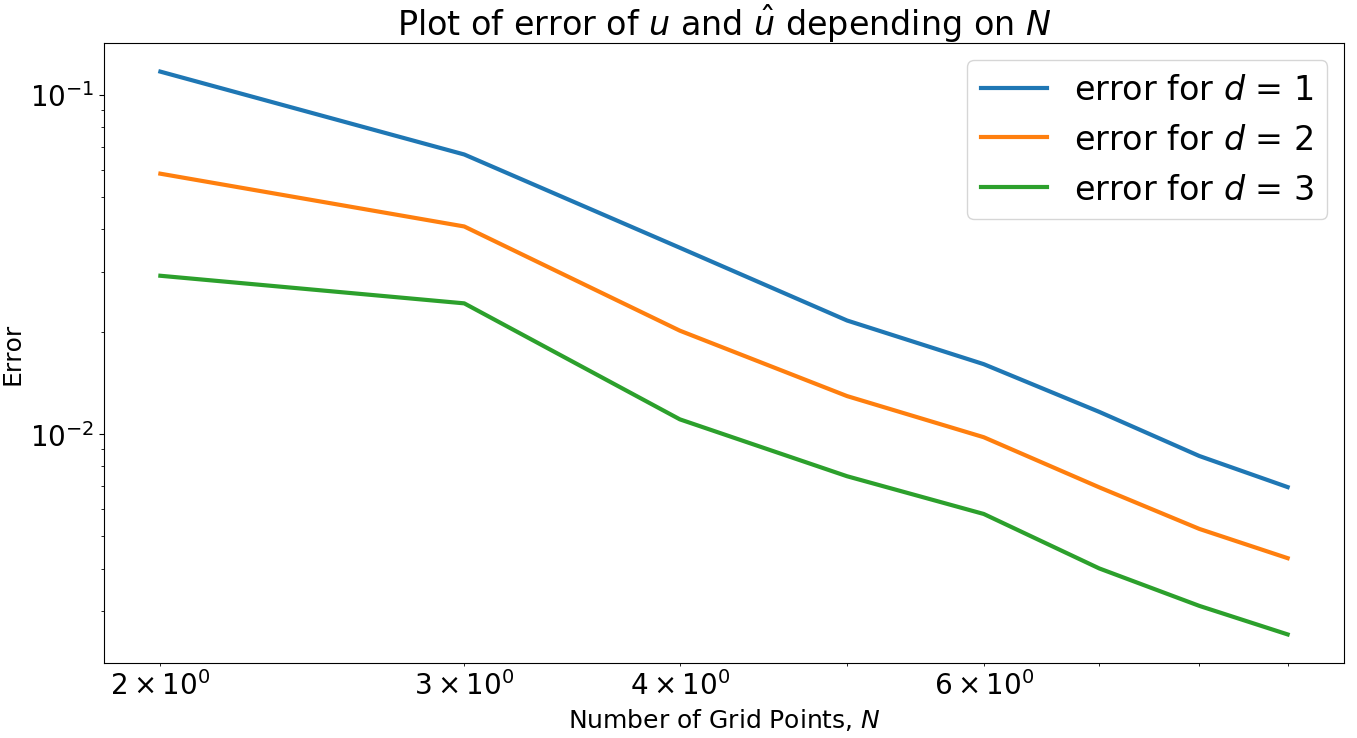
\includegraphics[width=\linewidth]{graphics/error_plot_sor.png}
	\caption{The Error for SOR}
	\label{fig:boat1}
\end{figure}

We can further ask, if the successive over-relaxation method converges faster than solving the system with the LU-decomposition. The visual comparison can be found at figure \ref{fig:boat2} (the plot is only for \(d = 2\) due to the limitation of the working computer of the authors).

\begin{figure}[h]
	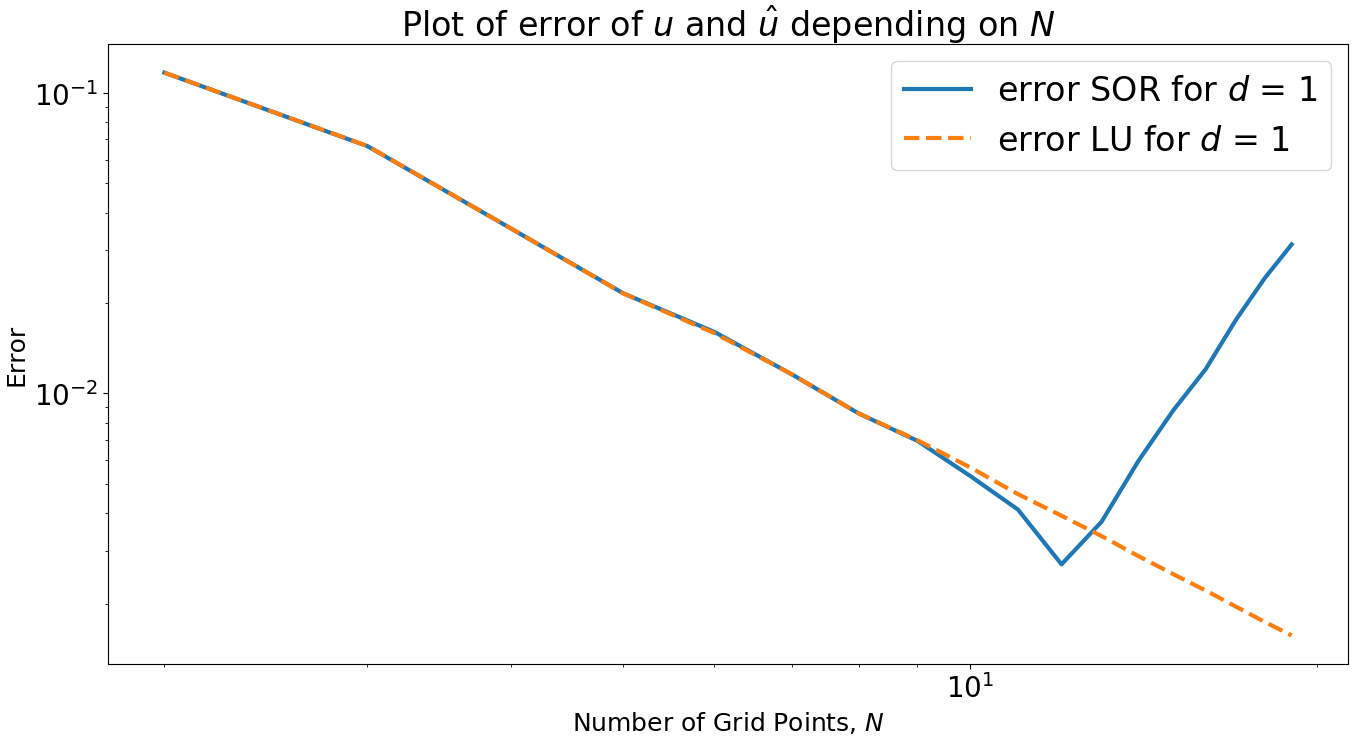
\includegraphics[width=\linewidth]{graphics/plot_error_both.png}
	\caption{The Error for SOR and LU}
	\label{fig:boat2}
\end{figure}

As one can see, the errors are similar on the left side, but at \(n = 12\) the successive over-relaxation becomes better. As the optimal value for \(\omega\) is dependent on \(N\), this means that the SOR algorithm is preferable to the LU-decomposition if a good \(\omega\) can be chosen.

\subsection{Effects of the Termination Condition}

In this section, we want to explore the change in the error plot if we alter the termination condition. Specifically, what happens when we choose \(\epsilon = \frac{1}{N + 1}^k\)? For this protocol, we will evaluate for \(k = 1, 2, 4\) and \(-2\).
If \(k = 2\), we get the following graph on figure \ref{fig:boat3}.

\begin{figure}[h]
    \begin{center}
	    \includegraphics[width=\linewidth]{graphics/plot_comb2.png}
        \caption{The Error for SOR and LU}\label{fig:boat3}
    \end{center}
\end{figure}

It is clear that in this case the error converges with the speed of \(\frac{1}{n^2}\). This leads us to believe that the speed of convergence is simply \(\frac{1}{n^k}\), but this turns out to be quite false. If we take \(k = 1, 4\), we get the plots on figure \ref{fig:boat3}.

As one can see, for \(k = 4\) the speed of convergence is still \(\frac{1}{n^2}\) while for \(k = 1\) it is simply \(n\).

This leads us to believe that for all \(k \geq 2\) the speed of convergence stays \(\frac{1}{n^2}\).

Finally, what happens if \(k = -2\)? Then the termination condition is \(\epsilon = (N + 2)^2\) which should be met quite quickly. This assumption is confirmed in figure \ref{fig:boat3} which shows the error does not converge to \(0\) at all.
\end{document}